\documentclass[tikz]{standalone}
\usepackage[utf8]{inputenc}

\usepackage{pgf}
\usepackage{tikz}
\usepackage[UKenglish]{babel}
\renewcommand\P{\mathsf{P}}
\newcommand{\NP}{\mathsf{NP}}
\newcommand{\PSPACE}{\mathsf{PSPACE}}
\newcommand{\PH}{\mathsf{PH}}
\newcommand{\co}{\mathsf{co}}
\newcommand{\F}{\mathsf{F}}
\newcommand{\DeltaP}[1]{\Delta^\P_{#1}}
\newcommand{\SigmaP}[1]{\Sigma^\P_{#1}}
\newcommand{\PiP}[1]{\Pi^\P_{#1}}

\usetikzlibrary{calc}
\begin{document}
	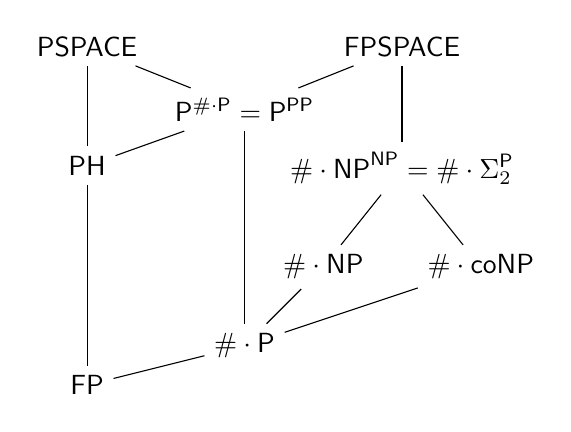
\begin{tikzpicture}

%				\fill[black!20!white,rounded corners] (-3.5,0) rectangle (3.5,6.5);
%				\fill[black!20!white] (-3.5,-.5) rectangle (3.5,1);
				
%				\fill[white] (-3.5,-0.52) parabola bend (0,.4) (3.5,-0.52);
%				\fill[white] (-3.5,-6.8) rectangle (3.5,-0.5);
					

	  			\node 	(FP)     	at (0,0) 					{$\F\P$};
				\node 	(numberP)   at (2,.5) 					{$\#\cdot\P$};	
				\node 	(numberNP)   at (3,1.5) 					{$\#\cdot\NP$};	
				\node 	(numbercoNP)   at (5,1.5) 					{$\#\cdot\co\NP$};	
				\node 	(numberNPNP)   at (4,2.75) 					{$\#\cdot\NP^\NP=\#\cdot\SigmaP2$};	
								
				\node (PH)			at (0,2.785) 				{$\PH$};
				\node (PSPACE)	at (0,4.3) 				{$\PSPACE$};
				\node (FPSPACE)	at (4,4.3) 				{$\F\PSPACE$};
				\node (PtonumberP)	at (2,3.5) 				{$\P^{\#\cdot\P}=\P^{\P\P}$};


				\path[-]
				(PH)	edge	(PSPACE)
						edge (PtonumberP)
				(PtonumberP) edge (numberP)
							 edge (FPSPACE)
				(numberP) edge (numberNP)
						  edge (numbercoNP)
				(numberNP) edge (numberNPNP)
				(numbercoNP) edge (numberNPNP)
				(FP) edge (PH)
				(FP) edge (numberP)
				(numberNPNP) edge (FPSPACE)
				(PtonumberP) edge (PSPACE);
							
							
			



%				\draw[draw=black!20!white,thick,rounded corners] (-3.5,-6.8) rectangle (3.5,6.5);
%				\draw[dashed,-]	(-3,0) parabola bend (0,.7) (3,0);
				
%				\node[rotate=90] at (3.2,4) {intractable};
%				\node[rotate=90] at (3.2,-3) {tractable};

		\end{tikzpicture}
\end{document}